\chapter{Details of the Monte Carlo Code}\label{chp:chp2}

%\begin{flushright}
%  {\em QUOTE GOES HERE }\\
%
%\ \
%
%\normalsize
%{AUTHOR}  
%\end{flushright}


\section{Monte Carlo Methods}
	 The name 'Monte Carlo' describes a class of modelling techniques that employ a stochastic approach to simulating mathematical and physical situations that are otherwise difficult or impossible to solve.  By repeatedly sampling random numbers from a probability distribution, numerical results to non-analytic problems may be obtained.  The approach was first used by researchers at Los Alamos in the late 1940s who adopted the method to model the transport of neutrons.  It is from the code name for this project, 'Monte Carlo', that the methods derive their name.  
	 
	 As the available computing power increased over the following decades, Monte Carlo methods became more and more useful as a means of solving complex problems and are now used widely across numerous fields including mathematics, statistics, engineering, finance, the physical sciences and many others.  The nature of the approach means that they are particularly well-suited to problems with multiple degrees of freedom, and especially when any of these degrees are coupled.  By using random numbers to represent quantities that parametrize a physical problem, a model may be generated that simulates a solution to the problem using a pseudo-random number generator.   It must be the case that the quantities that characterize the problem may be represented by a continuous distribution in the range [0,1] in order that randomly generated numbers may be translated into physical properties.  
	 
	 For each randomly-generated input, the model of interest is applied and an output - a 'possible outcome' - is obtained.  By iterating this process many times with randomly-generated inputs each time, many possible outcomes are generated and a probability distribution may be built up.  The interpretation of the outputted probability distribution is dependent on the manner of utilisation of the Monte Carlo method.  For example, the iterative procedure may be used to determine best-fitting parameters of a model or may be used to find the mean-free path of a photon.  In the former case, the multi-dimensional probability distribution may be analysed to determine the most representative model or models whereas in the latter case the probability distribution is equivalent to an energy distribution.
	 
	 Clearly, Monte Carlo simulations are limited by their finite nature and will never produce a perfect solution.  However, this does not mean that Monte Carlo simulations are lacking in rigour.  It may be shown that the error in a Monte Carlo model is approximately $\sim \frac{1}{\sqrt{n}}$ for large $n$, where $n$ is the number of quanta used in the simulation.  The error may therefore be made as small as required by increasing the number of quanta used in the simulation subject to the restrictions of computing time and expense.
	 
	 In the next section, I discuss the use of Monte Carlo methods as applied to radiative transfer problems and  specifically to DAMOCLES.  I discuss the computational aspects of my work and the architecture of the code in section \ref{damocles_struct} before finally discussing the limitations of the code and its potential for future developments in section \ref{limitations}.
	 
\section{Radiative Transfer and the Monte Carlo Method}
\label{rt}

 The application of Monte Carlo codes to radiative transfer problems in astrophysics has a strong history.  Numerous codes that utilise this stochastic methodology have been written in the past few decades in order to model the transport of photon packets through various media.  The energy to be transported throughout the region of interest is discretised into packets and the path of each packet is calculated according to the properties of the environments that it passes through during its lifetime.  Collating the escaped packets at the end of the simulation produces an energy distribution. 

There exist several Monte Carlo radiative transfer codes that use this technique in order to model the transfer of line emission through a nebula to produce a synthetic spectrum. There also exist a number of codes that treat the continuous emission and absorption of energy in dusty environments in order to produce and fit a spectral energy distribution (SED).  Models of supernovae have been produced using both approaches and well-fitting spectra and SEDs have been generated but never, according to the best of my knowledge, has the mechanism been employed to produce sophisticated models of line profiles in expanding dusty regions.  In this new code, we seek to apply the technique to an expanding dusty medium in order to consider the effects on a single emitted line profile.

Previous work by Leon Lucy has considered the problem of dust-induced asymmetric line profiles in the ejecta of supernovae and he has published results derived both analytically and using simple Monte Carlo simulations.  These simulations appear to be the only published instances of a numerical approach to studying this spectral feature.  The DAMOCLES code adopts the same approach as the original modelling by Leon Lucy but allows for a considerably more complex treatment of the composition, geometry and motion of the dusty medium.

Radiative transfer methods as applied to supernovae generally treat a wide wavelength range and seek to conserve the total energy.  In the case of SED modelling, this is often achieved by dividing the total energy into packets of equal weight and equal energy and iteratively determining the temperature and ionization structure.  In this work, the approach we adopt is somewhat simpler as only a very narrow wavelength range need be considered.  Rather than seeking to conserve the total energy, we assume that any packet absorbed by dust would be re-emitted outside the wavelength range of interest and thus no longer contributes to the resulting line profile.  Any absorbed packet is therefore removed from circulation.  In addition to this, the absorption and scattering of radiation by dust is independent of temperature and there is therefore no need to calculate temperatures throughout the nebula.  Similarly, in the case of radiative modelling of synthetic spectra of the ejecta of supernovae, approximations such as the Sobolev approximation are often employed to handle the blending of lines more efficiently.  This is unnecessary here as only a single line or doublet is ever treated and a comparatively narrow wavelength range considered. 

The subtleties of the problem we consider here lie in the treatment of an atmosphere expanding as fast as 10\% of the speed of light.  Lorentz transforms must be carefully applied in order that packets experience the appropriate degree of frequency shifting at emission and at each subsequent scattering event.  In this respect, the code is analogous to Monte Carlo radiative transfer models of electron scattering published by \ref{}.  Indeed, similar features are observed in the outputs of both.

Throughout this section, I will describe the principles, assumptions and techniques adopted in the production of the DAMOCLES before I move on to address the mechanics and architecture of the code itself.
 
	\subsection{Dust Species}
	\subsection{Grain Sizes}
	\subsection{Doublets}
	\subsection{Clumping}
	\subsection{Electron Scattering}
	\subsection{Initialisation and the Grid}
	\subsection{Energy Packets}
	\subsection{Emission and Propagation}
	\subsection{Doppler Shifting and Weighting}
	
\section{The Structure of DAMOCLES}
\label{damocles_struct}
	\subsection{Fortran 90 and OpenMP Parallelisation}
	\subsection{Modular Architecture} %%%%%NEED TO RENAME THESE MODULES!!!
	\clearpage
	\begin{centering}
	\fbox{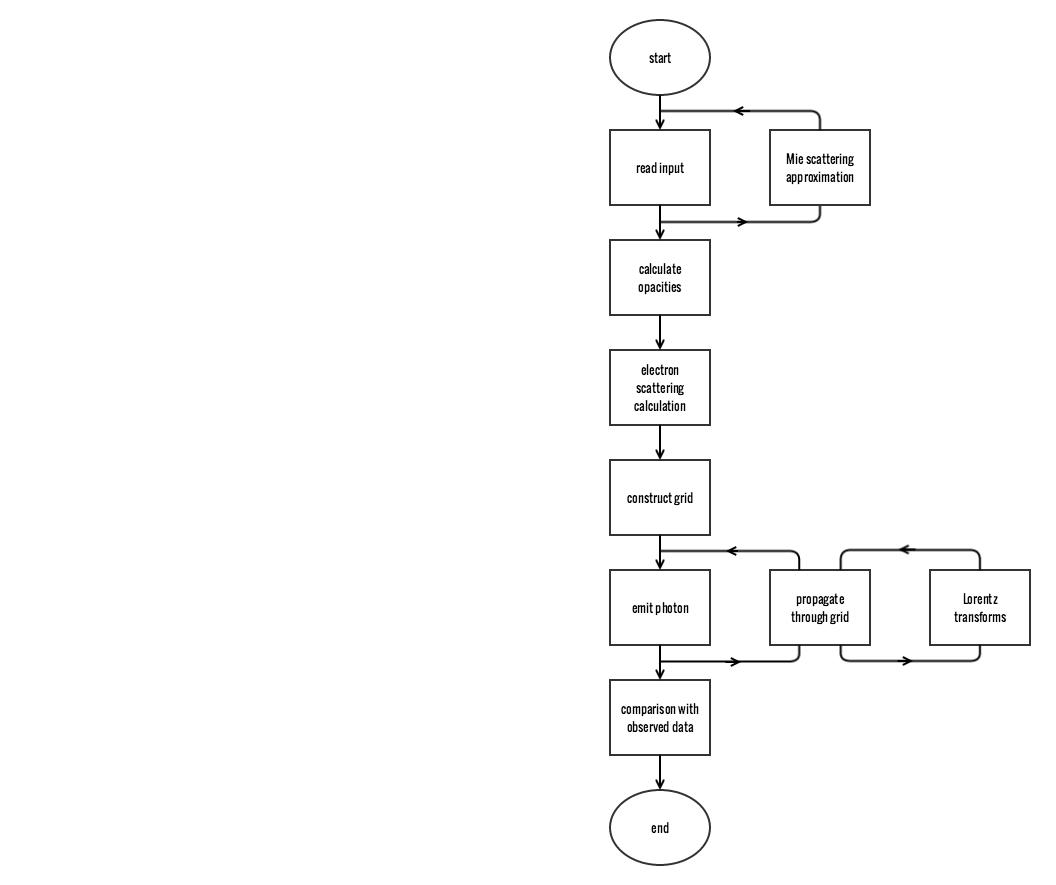
\includegraphics[scale=0.8, trim=200mm 0mm 0mm 0mm]{chapters/chapter2/code_flowchart.png}}
	\end{centering}
	\clearpage

		\subsubsection{Common}
		\subsubsection{Input}
		\subsubsection{Electron Scattering}
		\subsubsection{Random Routines}
		\subsubsection{Functions}
		\subsubsection{Sizes}
		\subsubsection{Global}
		\subsubsection{Photon}
		\subsubsection{Iterate}
		\subsubsection{Construct Grid}
		\subsubsection{Linear Interpolation}
		\subsubsection{Code}
		\subsubsection{Damocles}
		
	\subsection{Input}
	\subsection{Output}
	\subsection{Post-Processing and Visualisation}
\section{Limitations and Further Developments}
\label{limitations}

\clearpage
The code is written in Fortran 95 and uses a Monte Carlo grid method to model the transport, absorption, scattering and Doppler-shifting of monochromatic energy packets  through a smooth medium of dust grains of any composition of multiple species for which optical data is available.  Each species has an independent, specifiable size distribution.  Through the use of volume filling factors (see section \ref{section:clumping}), the code also has the capacity to treat dense clumps of dust surrounded by a smooth inter-clump medium.  Monochromatic energy packets are emitted diffusely according to an adapted mass density distribution ($\rho\propto r^{-q}$) and their frequency recalculated according to a radial velocity profile ($v \propto r^l$ ) and the Doppler effect formula (see section \ref{sec:doppler} and appendix A).

Initially, the grid is constructed and the density of each cell calculated.  A frequency array is set up and opacities calculated (as a function of mass density) for each frequency bin using a Mie scattering routine.  Photon packets are then generated with an initial position and direction, propagated and moved through the grid until they are either absorbed or escape the supernova.  

The propagation direction of a packet is randomly sampled from an isotropic distribution in the comoving frame of the packet.  The fate of a packet depends upon the albedo and density of the dust in the cells it passes through.  If it fails to escape a cell then, by comparing a randomly-generated number to the albedo, it is determined whether the packet is absorbed or scattered.  If it is absorbed then it is removed from the simulation;  if it is scattered then it escapes the grid cell and passes to the next.  

Since the scattering grain is subject to a strong velocity field, the frequency of the packet must be recalculated at each scattering event.  The repeated scatterings a packet experiences as it moves through the dusty medium may therefore result in repeated shifts to its frequency, a process known as �velocity-shifting�.  Ultimately, the escaped packets are collected along a line of sight and their frequencies recorded to produce a line profile.  Further details of each step may be found below.
%
%The variable parameters of interest in the code are:
%
%\begin{itemize}
%	\item{the total dust mass}
%	\item{the power-law exponents of the velocity and density profiles}
%	\item{the grain size range and power-law size index}
%	\item{the maximum velocity of the ejecta}
%	\item{the clump volume filling factor}
%	\item{the density contrast of the clumps}
%\end{itemize}

DAMOCLES stands for \textbf{D}ust-\textbf{A}ffected \textbf{M}odels \textbf{O}f \textbf{C}haracteristic \textbf{L}ine \textbf{E}mission in \textbf{S} upernovae.

\subsection{The grid}
\label{section:grid}
The bounds of the grid, the required resolution and the exponent of the density profile are declared in the input file and read in by the code.  The inner and outer radii of the supernova ejecta and the total mass of dust to be modelled are also input and the density of each cell is calculated accordingly.  The density within any given cell is constant and the densities of all cells exterior to the shell structure of the supernova ejecta are set to zero. 
 
\subsection{Clumping}
\label{section:clumping}

The code has a limited capacity to treat clumps, although work expanding this capability is currently being undertaken.  The approach used to populate the grid with clumps is based on the methodology used in the MOCASSIN code \citep{moc1,moc2,moc3,moc4}.  Clumps are currently all equal in size and are set to be the size of a single grid cell.  Though this inherently couples the size of the clumps to the overall resolution of the grid, this issue will be addressed in future versions of the code in which adaptive gridding will allow for increased resolution in clumped areas and ultimately a clump size distribution will also be included.  At present however, the number of clumps is calculated as per a specified volume filling factor, and the location of these clumps distributed according to the smooth density profile using an iterative approach i.e. the probability of each cell being a clump is calculated according to its radius and the overall distribution, a random number is generated and compared to this probability.  If the random number is less than the calculated probability then the cell is assigned to be a clump.  Iterating this process corrects the initial under-sampling.  

The volume filling factor is defined as the fraction of the total volume of the supernova that is occupied by clumps.  All clumps have the same density and this is set according to the density contrast at the inner radius of the supernova.  The density contrast is set by the user and defined to be the ratio between the mass density of the clumps and the density of the inter-clump medium at the inner radius.

\subsection{Multiple grain sizes and opacity calculation}
\label{sec:multigrain}

A frequency grid is established centered on the frequency of the line to be modelled, which is declared in the input file.  Files detailing the grain size distribution and the optical data for the chosen dust species are also declared at the start of the code.  For each frequency and grain size pair, a Mie scattering routine uses this data to calculate the overall $Q_{abs}(\nu)$ and $Q_{sca}(\nu)$ by summing over the weighted grain sizes.  This value is then used in the calculation of the opacity of each grid cell, which determines the fate of any packets passing through it (see section \ref{transport}).  A Mie scattering routine is an appropriate approximation in this instance as it applies in the case of spherical scatterers where the diameter of the sphere is of the same order as the wavelength of the interacting photon.  The wavelengths of the lines of interest for this code (particularly 6563 \AA \:H$\alpha$ and 6300 \AA \:[OI])  are in the optical and near-IR  and wavelengths are therefore of the order of 0.3-1.0$\mu$m, as are dust grain radii.

\subsection{Multiple species}
Any dust composition may be used for which there is optical data available. The relative abundances of the species may be declared by the user and for each species a size distribution (with minimum and maximum grain size and distribution $n(a) \propto a^{-t}$) may be used.  For each species, the calculations described in section \ref{sec:multigrain} are applied and the derived opacities are summed over each species weighted according to their relative abundances.  

\subsection{Photon packet propagation and transport}
\label{transport}
The supernova ejecta is divided into shells and the number of packets to be emitted in each shell calculated according to the square of the local density i.e. the lines are assumed to be recombination lines.  Though 6300 \AA \:[OI] is in fact due to collisional excitation and not recombination, it is still reasonable to assume that the emissivity scales with $\rho^2$ since the densities treated are low in comparison with the critical density ($N_{crit} \sim 10^{-6}$cm$^{-3}$).  In the future, higher densities may be considered, in which case the emissivities will be adjusted accordingly (scaling with $\rho$ above the critical density). 

It is assumed for this model that the distribution of emitting gas is coupled to the dust distribution and the number of photons emitted is therefore scaled to the dust distribution declared by the user.  Note here that only dust and not gas is treated by the model.  For each packet a location within that shell and an initial trajectory is randomly sampled from an isotropic distribution such that 

\begin{equation*}
\begin{aligned}[c]
\phi=2\pi\eta
\end{aligned}
\qquad\qquad
\begin{aligned}[c]
 \cos (\theta)=2\xi -1
\end{aligned}
\end{equation*}
\\
where $0<\eta<1$ and $0<\xi<1$ are random numbers, $\phi$ is the azimuthal angle and $\cos (\theta)$ is the radial direction cosine.

The grid cell that the photon packet is located within is identified and the packet is propagated through the grid.  A random number $0<\xi<1$ is sampled and the optical depth $\tau$ is calculated as $\tau=-\log (1- \xi)$.  This is because the probability that the packet travels a distance $L$ without interacting is 
$P(L)=e ^{-n \sigma L}=e ^{-\tau} $
where $n$ is the number density, $\sigma$ is the cross-section of interaction and $ \tau = n\sigma L$ for constant $n$ and $\sigma$ (as in a grid cell).  Noting that the probability that a packet does interact within a distance $L$ is therefore $1-e^{-\tau}$, we may sample from the cumulative probability distribution to give: 

\begin{equation*}
\xi = 1 - e^{-\tau} \quad \implies \quad \tau=-\log (1-\xi)
\end{equation*}

The frequency of the photon packet and the mass density of the cell are then used to calculate the opacity of that cell and, using the fact that $n\sigma=\kappa\rho$, the distance L that the packet travels before its next interaction is calculated.  If this value is greater than the distance from its position to the edge of the cell then the packet is moved along its current trajectory to the cell boundary and the process is repeated.  If the distance is less than the distance to the boundary then an event occurs and the packet is either scattered or absorbed with a probability dependent on the albedo of the cell:  a random number is sampled and if this is less than the albedo then the packet is scattered, if not then it is absorbed.  The albedo is defined as 

\begin{equation*}
	a=\frac{\sigma_{sca}}{\sigma_{sca}+\sigma_{abs}}
\end{equation*}
\\
where $\sigma$ is the cross-section of interaction.

If the packet is absorbed then it is simply removed from the simulation.  This is valid since in practice the photon packet would be reemitted at a much longer wavelength than the range of interest for a single line in the optical or near-IR. If the packet is scattered then a new trajectory is sampled from an isotropic distribution in the comoving frame of the dust particle.  This trajectory is then converted to the observer's frame for the purposes of continuing the photon packet's transport through the dusty medium.  At the point of scattering the frequency of the packet is also recalculated according to the Doppler formula.  These calculations are performed using the Lorentz boost matrix (see appendix A for further details).  This process is repeated until the packet has either escaped the outer bound of the supernova ejecta or been absorbed.

\subsection{Doppler shifting}
\label{sec:doppler}

All photon packets are initially created in the rest frame of the emitter with a monochromatic frequency that is specified by the user.  However, at emission events and at every subsequent scattering event, the frequency of the packet is recalculated according to the Lorentz transforms.  A velocity profile is specified by the user in the form $v \propto r^l$ as well as a maximum velocity at the outer radius of the supernova.  When the packet is emitted and every time it is scattered, the radius of interaction is considered and the velocity of the dust grain at that radius calculated.  The frequency of the packet is then updated according to this velocity by applying the Lorentz transform matrix to the momentum 4-vector $\bf{P}$. For a detailed mathematical description, see Appendix A.

It is worth noting that if a constant mass loss rate is required, the exponent of the velocity profile and the exponent of the density profile are not independent.  A constant mass loss rate implies that $4\pi \rho vR^2  \propto k$, where $k$ is a constant, and thus for $v \propto r^l$ and $\rho\propto r^{-q}$, we require that $q-l=2$.  However,  it is possible that the supernova event may have induced a mass-flow rate that is not constant with radius and thus both exponents may be declared independently.

\subsection{Photon packet weighting}
The energy of a packet is calculated as $E=nh\nu$, where $n$ is the number of photons contained in it, $\nu$ is the frequency of those photons and $h$ is Planck's constant.  In Monte Carlo simulations that model non-moving atmospheres, packets are usually taken to be of constant energy.  When the frequency of the packet is altered after an event, the energy of the packet is kept constant and the number of real photons contained within it assumed to change.  However, in the case of dust scattering, the number of real photons is conserved and thus the energy of the packet is altered.  This is most easily achieved by weighting each packet over all the scattering events as:

\begin{equation*}
w=\prod_{scat} \frac{\nu'}{\nu}
\end{equation*}

\noindent where $w$ is the weight of the packet.  The final energy of each packet is then $E=wE_0$, where $E_0$ is the energy of each packet at emission.

%\begin{wrapfigure}[28]{r}{0.55\textwidth}
%\centering
%\subfigure{\includegraphics[scale=0.4, trim=10mm 3mm 10mm 25mm]{{bench_imgs/a2.0_b0.0}.pdf}}\quad
%\subfigure{\includegraphics[scale=0.4, trim=10mm 3mm 10mm 3mm]{{bench_imgs/a1.0_b2.0}.pdf}}
%\caption{\textit{Above:} the analytic result for a line profile with $\alpha=2.0$ and $\beta=0.0$, in blue.  The model results for these values are in green. \textit{Below:} the analytic result for $\alpha=1.0$ and $\beta=2.0$, in blue.  The model results for these values are in green.}
%\label{fig:bench3}
%\end{wrapfigure} 


\subsection{Doublets}

One of the lines in supernovae emission spectra that is frequently seen to be blue shifted is the forbidden [OI] doublet (e.g. SN1987A \citep{LucyEtAl89} figure \ref{fig:Lucy89_87A}).  DAMOCLES therefore has the capacity to treat doublets as well as single lines.  When a doublet is specified, both the initial wavelengths and the initial intensity ratio must be declared.  The code will create a wider frequency array than for a single line in order to accommodate both lines.  It will then model each line independently, adding the final fluxes of the lines to produce the desired doublet at the end of the modelling. 


\subsection{OpenMP Parallelisation}



Monte Carlo photon transfer codes lend themselves particularly well to parallelisation since the trajectory of each packet is unaffected by the paths of the others.  Each processor can therefore calculate the paths of a set of packets dividing the transport workload linearly amongst the processors. The properties of all the packets can be collated when all packets have been processed through the nebula.  This is beneficial as it may considerably decrease the runtime of the simulation, which is particularly useful in cases of high optical depth.  The code was parallelised using OpenMP, a shared-memory parallelisation language compatible with Fortran and C programming languages. 
		
\noindent{FIRST PARAGRAPH}

THE REST FOLLOW HERE. 


